\section{Hardwarearkitektur}
Dette afsnit beskriver arkitektur for hardware i AutoGreen.

Forsyning til alle blokke er beskrevet på IBD for system, Figur \ref{fig:ibd_system_forsyn}. Forsyninger er ikke tegnet ind på øvrige diagrammer for overskuelighedens skyld. Det gælder desuden at alle blokke har fælles reference (GND). 

\clearpage

\subsection{BDD for System}
\begin{figure}[h]
\centering 
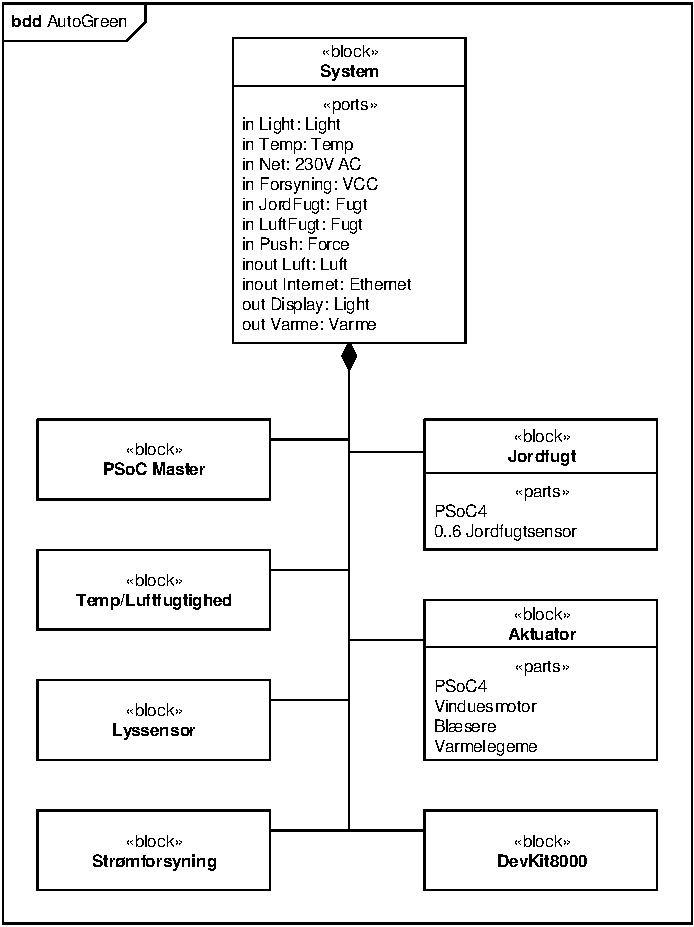
\includegraphics[width={\textwidth-2cm}, trim=0 0 0 0, clip=true] {../fig/bdd_system.pdf}
\caption{BDD for System.}
\label{fig:bdd_system}
\end{figure}
\clearpage

\subsection{IBD'er for System}

\begin{figure}[h]
\centering 
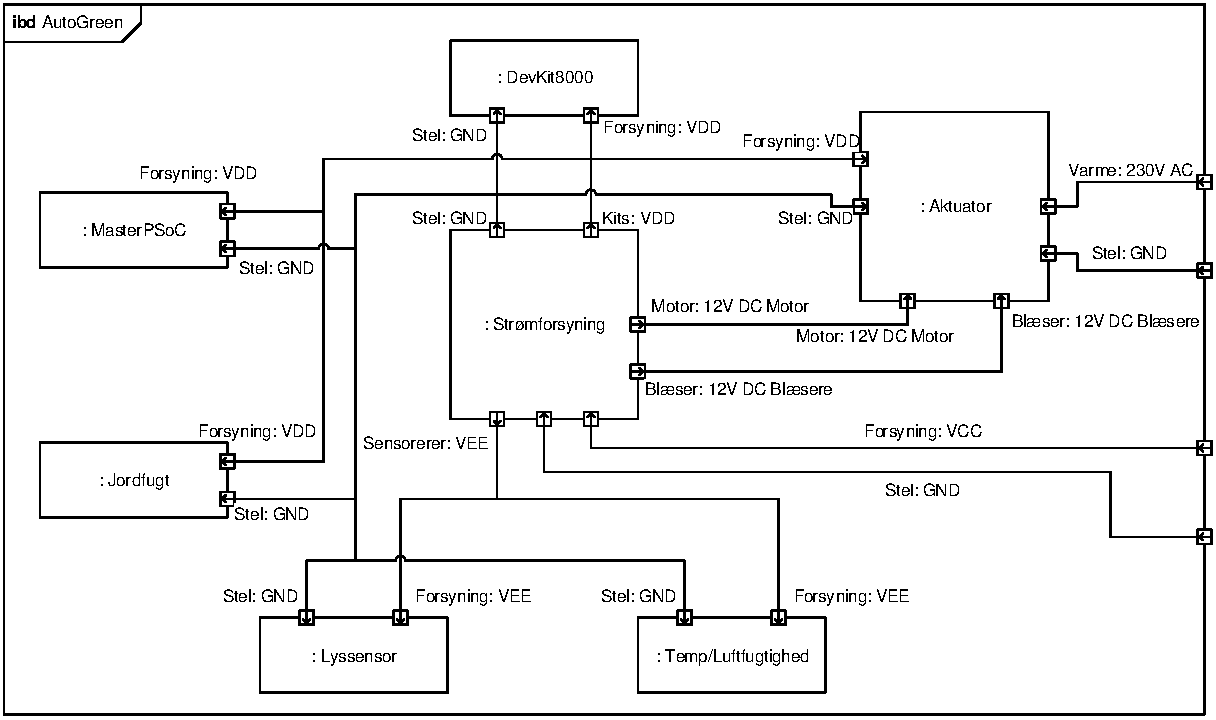
\includegraphics[width={\textwidth-2cm}] {../fig/ibd_system_forsyninger.pdf}
\caption{IBD for forsyninger i systemet.}
\label{fig:ibd_system_forsyn}
\end{figure}

\begin{figure}[h]
\centering 
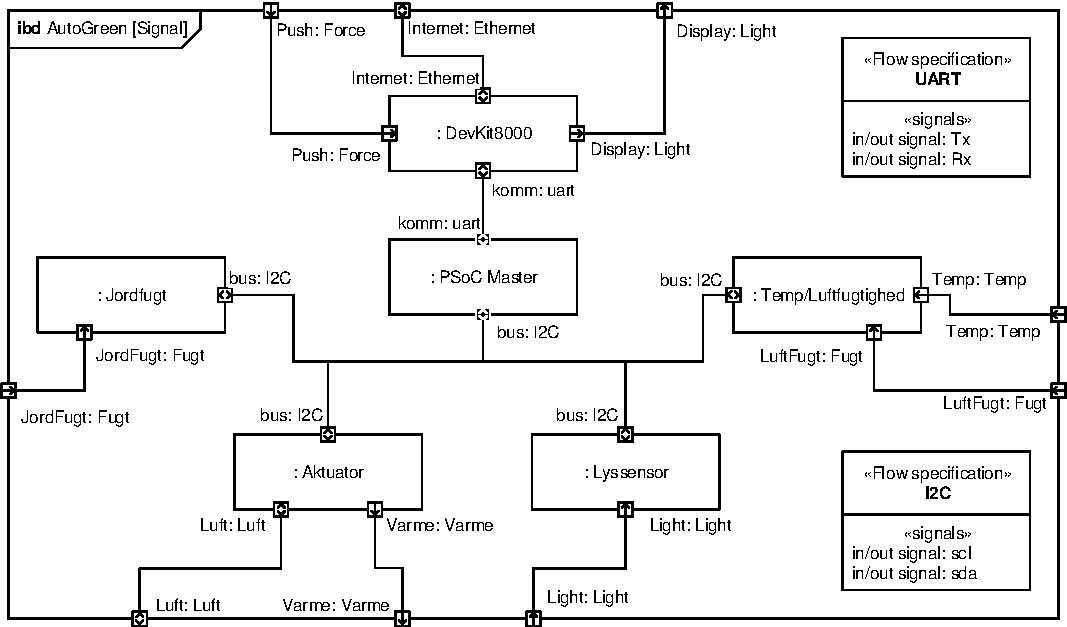
\includegraphics[width={\textwidth}-2cm] {../fig/ibd_system_signaler.pdf}
\caption{IBD for signaler i systemet.}
\label{fig:ibd_system_signal}
\end{figure}



\subsubsection{Strømforsyning}
Forsyner øvrig hardware i systemet, undtagen varmelegemet, Devkit8000 samt \IIC sensorer. Blokken forsynes fra en laboratorieforyning.
\subsubsection{DevKit8000}
Systemets brugerflade, er samtidigt controller for systemet. 
\subsubsection{MasterPSoC}
PSoC4 Pioneer Kit, der har til opgave at kommunikere via UART med DevKit8000 og via \IIC med slaver.  
\subsubsection{Temp/Luftfugtighed}
Denne blok indeholder en sensor med \IIC interface og måler temperatur og luftfugtighed i det fysiske drivhus.
\subsubsection{Lyssensor}
Består af en sensor med \IIC interface og måler lysintensitet i det fysiske drivhus. 
\subsubsection{Jordfugt}
Denne blok indeholder op til seks analoge jordfugtsensorer, som vha. et PSoC4 Pioneer Kit er koblet på systemets \IIC bus.
\subsubsection{Aktuator}
Denne blok indeholder et PSoC4 Pioneer Kit, der fungerer som \IIC slave og styrer systemets aktuatorer. 

\subsection{IBD for Aktuator}

\begin{figure}[h]
\centering 
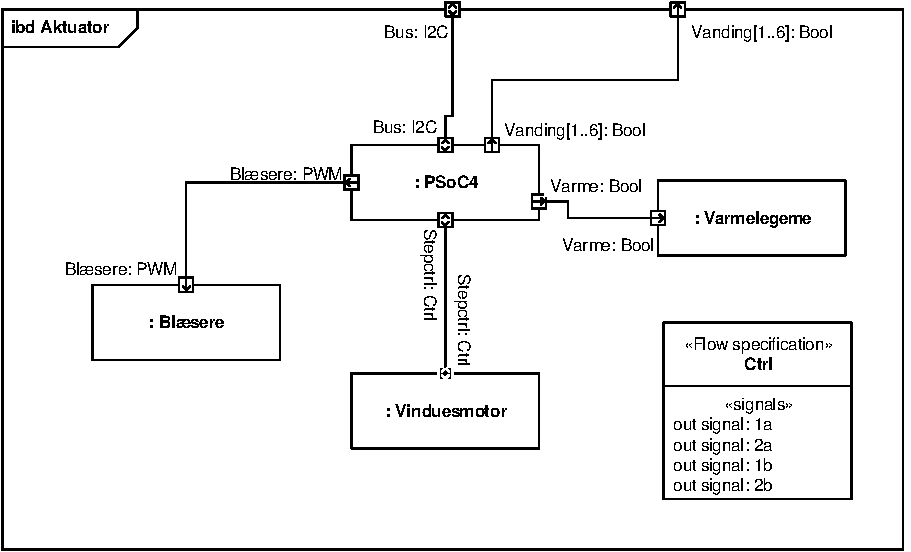
\includegraphics[width={\textwidth}, trim=0 0 0 0, clip=true] {../fig/ibd_aktuator.pdf}
\caption{IBD for Aktuator}
\label{fig:ibd_aktuator}
\end{figure}

\subsubsection{PSoC4}
PSoC blokken består af et PSoC4 Pioneer Kit, der agerer slave på \IIC bussen. 
\subsubsection{Vinduesmotor}
Denne blok består af en steppermotor, der styrer vinduet i det fysiske drivhus.
\subsubsection{Varmelegeme}
Varmelegeme med formål at hæve temperaturen i det fysiske drivhus. Varmelegemet styres af PSoC4 blokken, og det forsynes direkte fra elnettet (230V AC). 
\subsubsection{Blæsere}
Denne blok består af nogle blæsere, som kan ventilere luften i det fysiske drivhus. Blæserne styres af PSoC4, og de forsynes fra Strømforsyning. 

\subsection{IBD for Jordfugt}

\begin{figure}[h]
\centering 
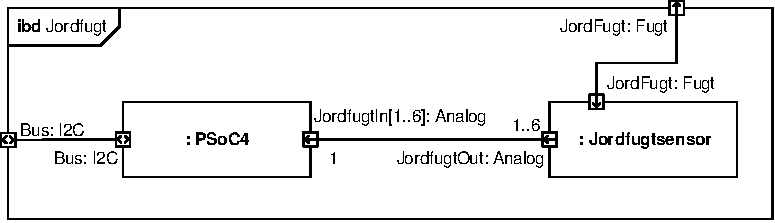
\includegraphics[width={\textwidth}] {../fig/ibd_jordfugt.pdf}
\caption{IBD for Jordfugt}
\label{fig:ibd_jordfugt}
\end{figure}

\subsubsection{PSoC4}
PSoC4 Pioneer Kit, der agerer slave på \IIC-bussen. 
\subsubsection{Jordfugtsensor}
Denne blok indeholder en analog sensor, der måler jordfugt ved en plante i det fysiske drivhus. Der kan kobles op til seks af disse til PSoC4.

\subsection{Signalbeskrivelser}

\LTXtable{\textwidth}{Systemarkitektur/HWarkitektur/signalbeskrivelser.tex}

\clearpage